\chapter{Ensembles of Stretchable Models} \label{sec:stretchable}
\section{Introduction}


In this chapter, we focus on the task of estimating and tracking articulated 2D 
human pose in videos ``in the wild'': single-view, uncontrolled settings 
typical in movies, television and amateur video.   Reliable
parsing of human motion in such videos could vastly improve and refine action 
recognition and semantic retrieval. This task is made difficult by the 
considerable background clutter, camera movement, motion blur, poor contrast, 
body pose and shape variation, as well as illumination, clothing and appearance 
diversity. There has been an explosion of recent work on articulated pose 
estimation from single images of this type~\citep{ronfard02, 
miko04,felz05,ramanan06,ferrari08,eichner09, andriluka09}, and the model 
proposed in~\secref{CPS}.  

Despite steady advances, localization of the most interesting parts (lower arms 
and hands) remains very inaccurate.  Video provides additional motion cues, yet 
most work on articulated tracking requires manual initialization from a few
frames~\cite{cardboard02,bregler98,balan06,sminchisescu03,ren07,buehler08}.  
Several recent papers~\cite{sigal04, lan05,ramanan05,ferrari08,weisssapp10}, 
however, combine tracking and estimation without any supervised initialization; 
our work in this chapter follows this setting, which we call {\em articulated 
motion parsing}.

\begin{figure}[t!]
\centering
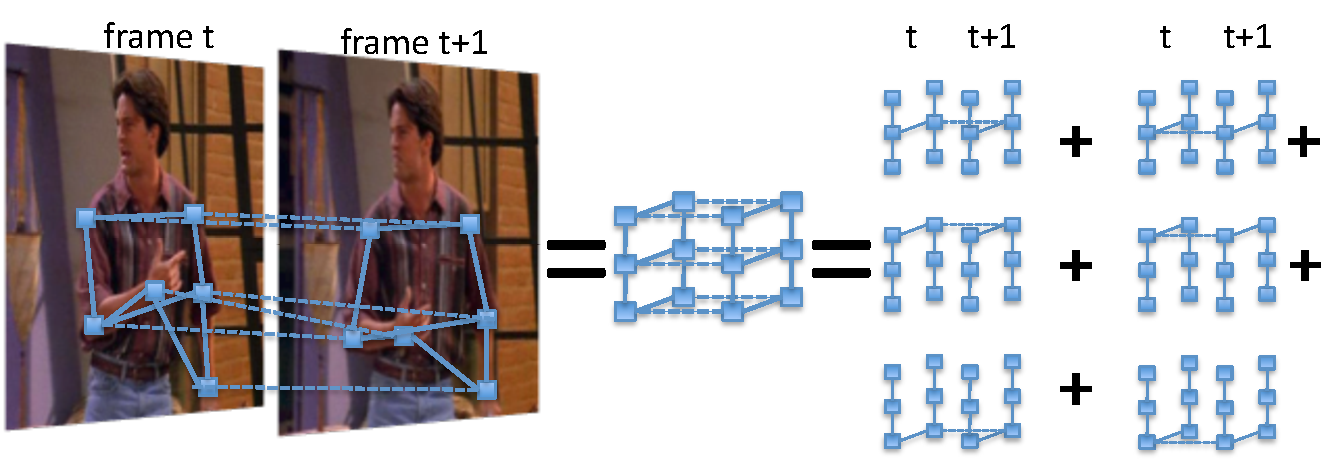
\includegraphics[width=0.99\linewidth]{figs/stretchable-overview.pdf}
\caption[Stretchable Ensembles overview]{\label{fig:overview} Overview.  On the 
left, we show a full model with edges representing all pairwise relationships 
we want to capture within and between frames.  We approximate this full, 
intractable loopy model by decomposing it into an ensemble of six models which 
cover the edge relationships of the full model.  Our joint-centric 
representation is considerably more flexible in modeling pose variability than 
rigid limb-based 
representations~\cite{ferrari08,sapp2010cascades,andriluka09}.}
\label{fig:stretchable-overview}
\end{figure}

% Intractability, loopy, sampling, etc..
In the ``strike-a-pose'' parsing method of~\cite{ramanan05}, an easily 
detectable canonical pose (e.g., limbs spread out) is automatically found in a 
long stretch of video and used as initialization for person-specific part 
appearance models.  While this intuitive idea works well when every person 
strikes the easy canonical pose at least once in every video, many motion 
sequences are short and all the poses are difficult.  Most work to date on 
short, difficult motions does not show significant improvement over single 
frame parsing~\cite{ferrari08,weisssapp10}, and sometimes causes actual 
degradation in accuracy when pose estimation is coupled across frames.
One crucial reason for this is that joint parsing of multiple articulated parts over time involves  intractable inference and learning problems, since part location/orientation variables have very large state spaces and the models are highly inter-connected  (high-treewidth). Because of this barrier, previous work has resorted to approximate inference using sampling~\cite{wang07,isard98,sminchisescu03,sigal04} and variational~\cite{sigal2004tracking,ferrari08} methods, which often introduce poorly understood error and/or bias.
The computational complexity of learning such models often limits the ability 
to learn rich features, resulting in using only simple, image-independent 
location-persistence coupling~\cite{ferrari08}.  %BT: Note that sigal04  actually has nice features.
One notable contrast to this is the work of~\cite{ren07}, which uses powerful 
image cues and inference to establish correspondences between frames and within 
frames.  However, their method makes greedy decisions  as it proceeds through 
frames in order to handle the intractability of maintaining a distribution of 
beliefs throughout the video sequence, and hence has no way of recovering from 
bad choices in earlier frames.


Computational considerations also usually lead to restrictive simplifying 
assumptions on geometry: 2D limb lengths are fixed (given global 
scale)~\cite{ramanan05,ferrari08,eichner09, andriluka09}.  In typical video 
sequences this assumption is almost always violated because of foreshortening 
and body type variation, especially for the lower arms. For this paper, we 
collected a new challenging video dataset which extends the one 
in~\cite{weisssapp10}, which we call VideoPose2.0.  In VideoPose2.0, roughly 
30\% of all lower arms are significantly foreshortened;  see 
Figure~\ref{fig:dataset} for a summary of the dataset variability.

In this work, we overcome these computational and modeling limitations
using an ensemble of tractable submodels which couple
locations of body joints within and across frames using rich
image-dependent cues.  We address the problems of foreshortening and
part scale variation by using joint centers (shoulders, elbows,
wrists) as parts~\cite{lee06,urtasun08,rogez08}, instead of
limbs. Each submodel in the ensemble tracks a
single joint through time (e.g., left elbow), and also models the
spatial arrangement of all joints in a single frame.  Because of the
tree structure of each submodel, we can perform efficient exact
inference and use rich temporal features that depend on image
appearance, e.g., color tracking and optical flow contours. The models
are trained discriminatively using a large-margin loss, and we
experiment with a range of inference techniques that introduce
increasing coupling between models (and thus increasing computational
cost). Intriguingly, we find that a highly efficient method of
enforcing agreement on single variables that we introduced in
\cite{weisssapp10} outperforms costly approximate inference using dual
decomposition.

\begin{figure}[tb!]
\centering
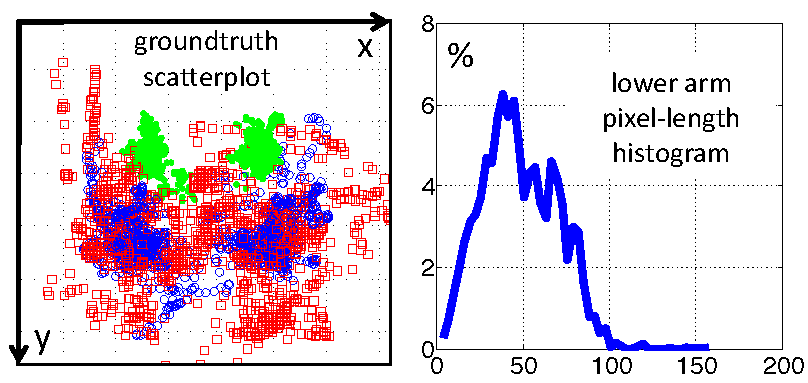
\includegraphics[width=0.9\linewidth]{figs/videopose-dataset-stats.pdf}
\caption[VideoPose2.0 statistics]{\label{fig:dataset} A summary of our new 
video dataset, VideoPose2.0.  \textbf{Left:} A scatter plot of groundtruth 
joints (green dot = shoulder, blue circle = elbow, red square = wrist).  
\textbf{Right:} Histogram of lower arm lengths in our dataset, illustrating how 
important it is to model relative part length in a real world setting.  }
\label{fig:videopose-dataset-stats}
\end{figure}

%jointly using a simple but effective 
%relaxation that results in linear scaling in complexity with the number of 
%parts.  

\out{
Our earlier work~\cite{weisssapp10} first investigated an ensemble of models 
for tracking body parts, but with several key differences: the model is 
designed to simply prune away unlikely hypotheses for torso and shoulder
locations, whereas in this work we focus on predicting the location of 
shoulders, elbows and hands---a significantly harder task.  Furthermore, like 
other previous work, \cite{weisssapp10} shows only a small improvement over 
single-frame parsing, and likewise the only temporal cue used is geometric persistence.
}

We apply our motion parsing model on a new video dataset of highly varied and 
articulated poses from TV shows containing over 1,200 frames.  We show 
significant quantitative and qualitative improvements over state-of-the-art 
single-frame pose estimation approaches (in particular, wrist and elbow 
accuracy improves by greater than 15\%).  In summary, the novel contributions 
of this work are: \textbf{(1)} an efficient ensemble of tree models for parsing 
human motion which covers a complex set of pairwise relationships and includes 
rich, image-dependent features; \textbf{(2)} stretchable 2D layout models, as 
opposed to the rigid parts typically used in pose estimation;
\textbf{(3)} significant improvement over single frame parsing results 
(arguably a first in this setting) \textbf{(4)} a challenging new video dataset, VideoPose2.0, 
with a high degree of motion pose variability which shows limitations of 
state-of-the-art methods.  The VideoPose2.0 dataset, code and videos are available at 
\textit{http://vision.grasp.upenn.edu/video}.



\section{Modeling}\label{sec:model}
As discussed, due to the intractability of jointly tracking multiple objects through time, previous 
work has made limiting assumptions in both the representation of pose (i.e., 
the inability to model foreshortening or fine angular granularity), and the 
interactions between parts, which do not capture rich, image-dependent 
relationships.  We address each of these issues in a principled framework.

\subsection{Stretchable models of human pose}  One of the biggest limitations 
of current models of human pose is the ``cardboard people'' 
assumption~\cite{cardboard02}: that body parts are rigid patches of fixed size 
(up to a global scale).  In the Pictorial Structures framework, the human is 
represented as a collection of parts with fixed lengths, which along with the 
position and angle of each joint, completely determines the pose of the 
person~\footnote{The seminal work of Felzenswalb et al.~\cite{felz05} uses 10 
discretized scales per part, but all modern implementations of PS use one fixed 
scale~\cite{sapp2010cascades,ferrari08,andriluka09}, partly due to its 
prohibitive increase in the state space.}.  Thus, wrists are always a fixed 
distance away from elbows in these models. This is a frequently violated 
assumption in realistic video, due to foreshortening and variation in body 
type.  In the VideoPose2.0 dataset we  introduce 
(Section~\ref{sec:experiments}), 30\% of lower arms are significantly 
foreshortened, see~\figref{videopose-dataset-stats}.

\mypar{Two joints $>$ one limb:} Rather than model human limbs as a position 
and orientation, we propose a model {\em directly on the pixel coordinates of 
each joint}.  Although this choice introduces more variables 
(one for each joint rather than for each part), the state space for each 
variable is drastically reduced because we no longer need to reason over a 
finely discretized set of angles in the state space, and we can now implicitly 
represent nearly any angle between parts.  In current PS implementations, this is a 
$24\times$ reduction in the state space of each variable.  In addition to 
this, because the length of the limb is now determined implicitly by the pixel 
distance between neighboring joints, the model naturally lends itself to 
capturing large variability in the part length.  Because of its ability to 
represent finely discretized limb length, we refer to this model as
{\em stretchable}, in contrast to the typical rigid, rectangle-based 
representation.

One side-effect of switching from a limb-centric to joint-centric model of 
pose is that unary attributes of the limb-centric model are now pairwise 
attributes of a joint-centric model.  Furthermore, pairwise attributes in a 
limb-centric model correspond to ternary attributes in a joint-centric model, 
which we do not use.  However, in a standard PS model, pairwise attributes are 
only image-independent functions of geometry, whereas in our model, pairwise 
potentials all incorporate image information, giving us overall a more 
expressive model than standard PS. 



\subsection{Ensembles of stretchable models (ESM)}
Ideally we want a model of human motion which captures important
relationships between all correlated parts.  This includes parts that
are connected kinematically (e.g., left elbow, left wrist), parts that
are left/right symmetric (e.g., left elbow, right elbow), and
instantiations of the same part in consecutive frames (e.g., left
elbow at time $t$, left elbow at time $t+1$).  Clearly, modeling all
these relationships together leads to cyclic dependencies
within a single frame (due to the three symmetry edges) and
between consecutive frames (due to the six tracking edges); 
see~\figreff{stretchable-overview}{left}. 

However, in general, it is always possible to express the score of a
given state assignment in a full, intractable model as the sum of
scores under a set of tree sub-models that collectively cover every
edge in the full model. This is the key insight that allows us to
include all the rich relationships we desire: we {\em decompose} our
model of all interesting relationships related to parsing human motion
into an ensemble of submodels, all of which are trees (and therefore
tractable). Each tree submodel is responsible for tracking a single
joint through time and additionally models the corresponding set of
pairwise interactions between joints in a single frame
(\figreff{stretchable-overview}{right}).

Formally, we pose this problem as a structured prediction task, where
the input $x$ is a video sequence of $\ell$ images and the output $y$ is a
sequence of $n\ell$ variables, where $n$ is the number of parts (joint
locations) included in the model. Each output $y_i$ is the 2D
coordinate of some part joint (defined in a $80 \times 80$
discretization of the pixel space) in some frame.  We also use the shortcut notation 
$y_{\bf t} = \{ y_i \;|\; y_i \text{ is in frame } t \}$
to index all $P$ joint variables in frame $t$.  

\out{
Given a training set
$S = \{(x^{(j)},y^{(j)})\}_{j=1}^n$ of samples from a joint
distribution, the standard supervised learning task is to learn a
hypothesis $h: X \mapsto Y$ that minimizes the expected loss $\E{S}{
  \cL\left(h(x^{(j)}) , y^{(j)}\right)}$ for some non-negative loss function $\cL
: Y \times Y \rightarrow \reals^+$. The linear hypothesis class we
consider is of the form $h(x) = \argmax_y \score{y}$, where the
scoring function $\score{y} \triangleq \w \cdot \f(x,y)$ is the
inner product of a vector of parameters $\w$ and a feature
function $\bft: X \times Y \mapsto \reals^d$ mapping $(x,y)$ pairs to
$d$ real-valued features.  }


Let $G = (\cV,\cE)$ be our full graphical
pose model; we further assume a general pairwise MRF model that decomposes over 
the vertices $\cV$ and edges $\cE$, so that
\begin{equation}
  \label{eq:loopy-model}
  \score = \sum_{i \in \cV}\w_i \cdot \f_i(x,y_i) + \sum_{(i,j) \in \cE}\w_{ij} 
\cdot \f_{ij}(x,y_i,y_j).  \end{equation}
Note that edges $(i,j)$ may connect variables between consecutive
frames. Let there be $P$ tree sub-models, and $G_p = (\cV, \cE_p)$ be the sub-graph of $G$ corresponding
to the $p$'th one as in~\figreff{stretchable-overview}{right}.  Then
we decompose the score $\score$ into the sum of the scores of the
$P$ constituent sub-models: $\score = \sum_{p=1}^P s^p(x,y)$, the
score of the $p$'th model is as in~\equref{loopy-model}, restricted to the
edges $\cE_p$, i.e. 
\begin{equation}
s^p(x,y) = \sum_{i\in\cV}\w_i^p \cdot \f_i(x,y_i) + 
\sum_{(i,j)\in\cE_p}\w_{ij}^p \cdot \f_{ij}(x,y_i,y_j).
\end{equation}
Note that we do not couple parameters across different models $\w^p$, so that different models can learn different parameters and effect different behaviors accorded to strengths and weaknesses dictated by their graph structures.

\out{
\begin{figure}[]
\centering

\includegraphics[width=0.9\linewidth]{figs/empty.jpg}
\caption{\small \label{fig:dd} Decoding with Dual Decomposition
  (examples). \textbf{Left:} The argmax predictions of each of the
  sub-models in the ensemble; note the disparity in predictions.
  \textbf{Right:} The prediction after running Dual Decomposition for
  500 iterations or until convergence (Yellow) compared to the
  predictions from \cite{sapp2010cascades} (Magenta).}
\end{figure}
}

\subsection{Inference}\label{sec:stretchable-inference}
We explore several methods for combining the $P$ independent models
during test time to make a single final decision.  The methods form a
hierarchy of agreement criteria between the submodels: at one extreme,
we enforce the constraint that all submodels must agree on the
maximizing assignment to all variables, and at the other, inference is
completely decoupled across submodels. Note that there is an inherent
trade-off between the degree of agreement imposed on the models and the
computational cost of the corresponding inference.  We present our
inference methods by order of decreasing agreement below.

\paragraph{Full Agreement via Dual Decomposition.} A natural goal is
to find the argmax decoding of joint locations throughout the entire
sequence of frames using our original model in~\equref{loopy-model}.  However, 
solving the argmax decoding problem
exactly is prohibitively expensive, due to the high treewidth of this
cyclic graph. We use the method of Dual Decomposition (DD)
\cite{bertsekas99,komodakis2007dualdecomp} to solve a linear
programming relaxation of the decoding problem as follows. Observe
that the argmax decoding problem of our full model can be decomposed
into $P$ subproblems { if those problems are coupled through a global
  equality constraint}:
\begin{align}
  \label{eq:dual-decomp}
&\argmax_{y, y^1,\dots,y^P} \sum_{p=1}^P s^p(x,y^p)  \textrm{ s.t. } \:  y^p=y  \quad{}\quad{(DD)}
\end{align}
Although the optimization \eqref{eq:dual-decomp} is still intractable because of the integral constraints, optimizing the {\em dual} of \eqref{eq:dual-decomp} is always
tractable (if we first drop the integrality requirement), but no longer guaranteed to return an optimal integral solution. We solve the dual problem with sub-gradient descent. Once complete agreement between all
$y^p$ is reached, then inference has converged to the exact solution
of \eqref{eq:dual-decomp} (although eventual convergence is not
guaranteed.) In our experiments, if dual decomposition did not
converge (after 500 iterations in practice, each requiring inference in all $P$ models), we used the maximum scoring primal variables found during
any descent iteration.

To solve the dual problem with sub-gradient descent, we introduce
Lagrange multipliers $\nu_{ik}^p$ for every possible state assignment
$y_i = k$ in every part model. We then alternate between updating the
dual variables $\nu^p$ and the primal variables $y^p$:
\begin{align}
  y^p & \leftarrow \argmax_y \left( s^p(x,y) +  \sum_{i,k} \nu^p_{ik} \ind{y_i=k^p}\right) \\
  \nu^p_{ik} & \leftarrow \nu_{ik} - \alpha\left(  \ind{y_i^p=k} - 
\frac{1}{P}\sum_{p=1}^P \ind{y_i^p=k} \right),
\end{align}
where $\alpha$ is a rate parameter chosen according to the scheme given in \cite{komodakis2007dualdecomp}.
 


\paragraph{Single Frame Agreement.} An alternative to computing the
MAP decoding of the entire sequence is to find the argmax solution
while constraining model agreement to only a subset of the variables
at a time.  If we restrict our attention to the variables in a single
time frame only, inference is considerably simpler.  For each frame
$t$, we solve
\begin{equation}
\argmax_{y_{\bf{t}}'} \sum_{p=1}^P \;\; \max_{y : y_{\bf{t}} = y_{\bf{t}}'} s^p(x,y) \quad{}\quad{(SF)}
\end{equation}
to obtain the joint configuration for that frame (remember $y_{\bf t}$
denotes the {\em set} of $n$ joint variables in frame $t$).  In words,
the inner maximization finds the highest scoring sequence $y$ subject to
the constraint that the variables in frame $t$ are fixed at positions
$y_{\bf t}'$.  The outer $\argmax$ is over all possibilities of single
frame configurations $y_{\bf t}'$.  This extends the notion of a
max-marginal of a variable (see~\secref{max-marginals}) to a max-marginal
over {\em a set} of variables.  This method requires first computing
the max-sum messages in a forward-backward message passing algorithm (see~\algref{mm-inference}), sent to variables in frame $t$, in each of the submodels.  Finding the argmax decoding of $y_{\bf t}$ is then
equivalent to inference in a grid with $n$ variables (in our case $n=6$
joints).  This can be solved exactly by forming cliques of size 3, for
which the message passing clique-tree forms a chain. The construction is 
illustrated in~\figref{single-frame-agreement}.  In each clique,
there are at most pairwise potentials, and since the state space of
each part is relatively small ($|Y_i| \leq 500$), the $O(\sum_i |Y_i|^3)$ cost 
of this inference takes less than a second per frame in
practice, and in our experiments took about as long as performing inference in 
all $P$ tree submodels (i.e., twice as slow overall).

\begin{figure}[tb]
\begin{center}
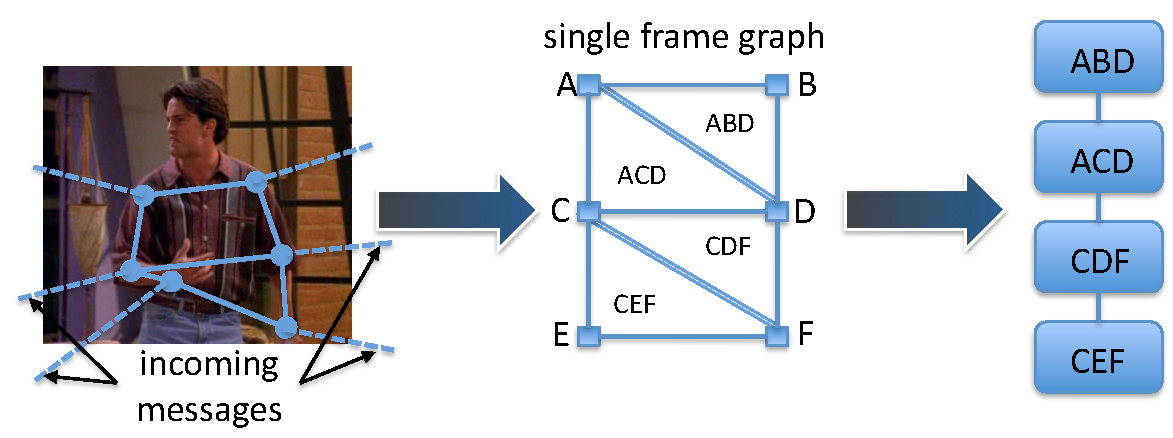
\includegraphics[width=0.99\textwidth]{figs/single-frame-agreement.pdf}
\caption[Single Frame Agreement construction]{Single frame agreement 
construction.  We first precompute messages coming into frame $t$ from all 
other frames (left).  We then combine 3-cliques state spaces via cartesian 
product to merge cliques into nodes in a larger state space (middle) to obtain 
a chain graph (right) over which we can perform exact inference.}
\label{fig:single-frame-agreement}
\end{center}
\end{figure}



\paragraph{Single Variable Agreement.} 

We can further narrow our subset of interest down to a single variable
at a time \cite{weisssapp10}.  This is a weaker criteria for model
agreement, but yields cheaper and simpler inference.  This gives us
the following inference problem for the $i^{th}$ variable:
\begin{equation}
\argmax_{y_i'} \sum_{p=1}^P \max_{y: y_i=y_i'} s^p(x,y) \quad{}\quad{(SV)}
\end{equation}
This can be solved by computing max-marginals for each model using standard forward-backward message passing, summing the $P$ max-marginal scores, and taking the highest scoring sum.
Note that this is actually equal to the best assignment decoding in the full 
model~\equref{loopy-model} {\em when all sub-models agree on the argmax}.  
However, this rarely occurs in practice.

\paragraph{Independent / No Agreement}
We also compared the above methods to predicting each joint using the single 
model in the ensemble that incorporated temporal dependencies for that
specific part, which we call the $Independent$ decoding scheme.


\subsection{Learning} Although we enforce agreement during ensemble inference 
at {\em test time}, coupling inference during training for more than one 
variable is prohibitively expensive to use as part of a learning procedure.  
Thus we learn
parameters $\w^p$ using {\em decoupled} inference separately for
each model. To learn parameters, we optimize a convex hinge-loss
objective for each model $p$ separately:
 \begin{align}
\min_{\theta_m} \frac{\lambda}{2}||\w^p||^2 +
\frac{1}{n}\sum_{j=1}^m \left[ \max_y s^p(x^{(j)},y) - s^p(x^{(j)},y^{(j)})
+1\right]_+
\end{align}
We optimize this problem via stochastic subgradient descent, as explained in 
\secref{learning}, and we choose
$\lambda$ and the number of training epochs using a held-out
development set to minimize error.



